


 \title{Third Week's Git Assignment} 

 \maketitle


\begin{abstract}
This document provide a brief introduction to Maximus' personal life, his goals, and his love for privacy.
\end{abstract}
\section{Background and Objectives for This Course}
Maximus a.k.a. \emph{"Cyber Gladiator"} works in the field of cybersecurity and is currently studying security this semester to focus on CPS/IoT designs, vulnerabilities, and flaws. As a student, he loves/ obsessed with privacy, and he hopes that he will become a more effective computer science researcher focusing on CPS/IoT systems by taking computer science research course this Fall.

Maximus' main area of interest includes (but not limited to) information systems’ vulnerabilities, vulnerabilities in system design and implementations, cyber risk assessment of IoT systems, and management of the risk in critical information systems in the broader context of their daily effects on individuals.


\begin{figure}[htbp]
\centerline{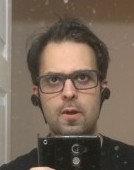
\includegraphics{a481.jpg}}
\caption{Maximus is currently looking at the mirror.}
\label{fig}
\end{figure}

Question 1: Have you focused any of your research in hardware vulnerabiilty specifically?  (from Cassandra Putman)  

Question 2: In regards to providing security to CPS/IoT systems; do you feel that the trends in FPGA systems could lend itself to provide energy-efficient security mechanisms without the need for complex environmental (eg network) requirements? (Many of the papers that I have seen lately have mentioned adding in monitoring systems for IoT networks, but that doesn't really scale to consumers. FPGAs could provide complex cryptographic mechanisms without the need for external systems.)